\documentclass[a4paper, 12pt]{article}
\usepackage{listings} 
\usepackage{xcolor}
\usepackage{mdframed}
\usepackage{graphicx}
\usepackage{pgfplots}
\usepackage{float}
\usepackage{mathtools}
\DeclarePairedDelimiter\ceil{\lceil}{\rceil}
\DeclarePairedDelimiter\floor{\lfloor}{\rfloor}

\definecolor{code-gray}{gray}{0.93}
\begin{document}
\title{ECE 341 - Lab \#8}
\author{Collin Heist}
\date{\today}
\maketitle
\pagenumbering{roman}
\tableofcontents
\lstlistoflistings
\newpage
\pagenumbering{arabic}

\section{Introduction}
The purpose of this lab is to create a \textit{library} of sorts, for interacting with a generic external memory device via $I^2C$. For this lab we'll be using the on-board \textbf{24LC245 EEPROM}. This library will be primarily used to read and write arbitrary lengths of data to said device. I'll be testing this library by creating two arrays both of equal but arbitrary lengths and data, writing that data to the EEPROM, reading that same data from the EEPROM, and then comparing the two arrays. Should my library be coded correctly, then the two arrays will be identical and that result will be displayed on the LCD.

Communicating with the EEPROM is done using $I^2C$, and rather than bit-twiddling the $I^2C$ module manually, I'll be using the $I^2C$ peripheral available on the \textbf{PIC32}. This peripheral makes using the $I^2C$ a lot easier, especially since the timing constraints of the communication are taken care of, so long as I properly use the \textbf{IdleI2C2()} function, which prevents the processor from stepping through all the $I^2C$ code faster than desired which results in failed communications.

The EEPROM does have some peculiarities that will influence the library I'll be writing. The most important thing is the page-latch limitation. This is a 64-byte long 'page' that temporarily keeps the data being written to the EEPROM's internal memory. Before the data is written to the EEPROM's actual memory, it is stored on the page-latch, and then a $I^2C$ stop initiates the transfer for the EEPROM. Should a page transition occur, meaning the data being written goes from one 'page' to the next, the writing wraps around to the beginning of the page (meaning the data's contiguity is lost). Because of this, my code takes close attention to provide stops and polling of the EEPROM whenever a page transition occurs.

\section{Implementation}
To start, the header file for the EEPROM communications:

	\begin{mdframed}[backgroundcolor=code-gray, roundcorner=10pt,
								innerleftmargin=5, innertopmargin=5, innerbottommargin=5]	
	\begin{lstlisting}[language=C, caption=EEPROM Library Header File, tabsize=2]
	#ifndef __I2C_EEPROM_LIB_H__
		#define __I2C_EEPROM_LIB_H__

		#define FSCK						400000
		#define BRG_VAL					((FPB / 2 / FSCK) - 2)
		#define PAGE_LEN				64

		#define WRITE						0
		#define READ						1

		#define CURR_MEM_ADDR					-1
		
		#define NO_ERR								0
		#define ERR_ZERO_LENGTH				1
		#define ERR_INVALID_MEM_ADDR	2
		#define ERR_INVALID_READ			3

		#define FALSE									0
		#define TRUE									1
	#endif

	// Function Prototypes
	...
	\end{lstlisting}
	\end{mdframed}
	
The first two macros are for setting the clock frequency of the $I^2C$ bus. This was provided in the previous lab, and I did not change any of these values for this lab. The value of \textbf{BRG\_VAL} will be used in the initialization function, and that's it.

Next, I defined two macros for write and read respectively. Their values are determined by the R/$\overline{W}$ line on the $I^2C$ data bus. For this, writes are \textbf{SDA} as a logical low, while reads are a logical high. These are macros to improve the readability of the library's code. The next section of macros are for specific cases and 'errors' in the library's code. The \textbf{CURR\_MEM\_ADDR} macro is negative to detect if, during a read sequence of the EEPROM, no address byte needs to be sent. The other macros are errors that could occur during either the read or write operations. Their names are pretty self-explanatory, but the lab description said to account for some of the possible fringe-cases of use during this library, which will be shown later. After the basic macros for boolean values and the function prototyping, the header file for the EEPROM library is finished.

\newpage
The first actual code I wrote was the initialization for the $I^2C$ peripheral. This is shown below:

	\begin{mdframed}[backgroundcolor=code-gray, roundcorner=10pt,
								innerleftmargin=5, innertopmargin=5, innerbottommargin=5]	
	\begin{lstlisting}[language=C, caption=$I^2C$ EEPROM Initialization Function, tabsize=2]
	void init_eeprom() {
		OpenI2C2(I2C_EN, BRG_VAL);
		IdleI2C2();
	}
	\end{lstlisting}
	\end{mdframed}
	
Clearly, this is a very easy task, using the peripheral library function to open $I^2C$ channel 2 on the \textbf{PIC32} is one function call using the enable macro and the clock speed defined in the header. One thing to note is that we're using channel 2 of the $I^2C$ bus, as that is internally wired to the EEPROM on our board. Then, the state of the bus is set to \textit{idle}, as this tells the processor to leave both \textbf{SDA} and \textbf{SCL} lines high, and sets the finite state machine to its proper state.

The next function is a 'helper' function of sorts, I used to improve my code's readability. Rather than having long conditional statements using the \textbf{\%} operator to determine if a number is divisible by another (in this case the page width), I wrote the following:

	\begin{mdframed}[backgroundcolor=code-gray, roundcorner=10pt,
								innerleftmargin=5, innertopmargin=5, innerbottommargin=5]	
	\begin{lstlisting}[language=C, caption=Multiple-of Function, tabsize=2]
	int is_multiple(int value, int multiple) {
		return (value % multiple ? FALSE : TRUE)
	}
	\end{lstlisting}
	\end{mdframed}
	
This is used in the code that \textit{writes} to the EEPROM, but to start off with the simpler function, this is the final 'helper' function I wrote for this library:

	\begin{mdframed}[backgroundcolor=code-gray, roundcorner=10pt,
								innerleftmargin=5, innertopmargin=5, innerbottommargin=5]	
	\begin{lstlisting}[language=C, caption=Sending an Arbitrary Control Byte, tabsize=2]
	int send_control_byte(int slave_addr,
		int mem_addr, int r_w) {
		
		int i2c_error = 0;
		int control_len = (mem_addr < 0) ? 1 : 3;
		int control_byte[3];
		control_byte[0] = slave_addr << 1 | r_w;

		if (control_len == 3) { 
			control_byte[1] = (mem_addr & 0xFF00) >> 8;
			control_byte[2] = mem_addr & 0x00FF;
		}

		int i = 0;
		while (control_len--)
			i2c_error |= MasterWriteI2C2(control_byte[i++]);

		return i2c_error;
	}
	\end{lstlisting}
	\end{mdframed}
	
This function is written to send an arbitrary control byte to the EEPROM. This function assumes that the communication has already been started (\textbf{StartI2C2()} was previously called), and it does not terminate the communication either, so that further read or write operations can occur. These control bytes address the EEPROM at a specific device address, and then can either send a memory address or not (depending on if a read is occuring). In this case, I use a negative memory address to denote that no memory address will be sent along with the control byte. The first byte of the control sequence is always the left-shifted slave address, following by a read or write, depending on which operation is occuring. The rest of the sequence is determined by if a memory address is being sent, if it is then the LSB and MSB are isolated and sent separately. Finally, the control byte is sent, and any errors are returned.

The first instance of this function being used is in the arbitrary read function, shown below:

	\begin{mdframed}[backgroundcolor=code-gray, roundcorner=10pt,
								innerleftmargin=5, innertopmargin=5, innerbottommargin=5]	
	\begin{lstlisting}[language=C, caption=Arbitrary EEPROM Read, tabsize=2]
	int read_eeprom(int slave_addr, int mem_addr,
		char* i2c_data, int length) {
		
		if (!length)
			return ERR_ZERO_LENGTH;

		if (mem_addr + length > 0x7FFF || mem_addr < 0)
			return ERR_INVALID_MEM_ADDR;

		int i2c_error = 0;
		StartI2C2();
		IdleI2C2();

		i2c_error |= send_control_byte(slave_addr,
				mem_addr, WRITE);
		RestartI2C2();
		IdleI2C2();
		i2c_error |= send_control_byte(slave_addr,
				CURR_MEM_ADDR, READ);

		if (i2c_error)
			return ERR_INVALID_READ;
	
		int index = 0;
		while (length-- > 1) {
			i2c_data[index++] = MasterReadI2C2();
			AckI2C2();
			IdleI2C2();
		}
		i2c_data[index++] = MasterReadI2C2();
		NotAckI2C2();
		IdleI2C2();
		StopI2C2();
		IdleI2C2();

		return NO_ERR;
	}
	\end{lstlisting}
	\end{mdframed}

This is a pretty large chuck of code, but it's actually quite simple. First, the error macros defined in the header file are used if the user is trying to read an either invalid amount of memory, or at an invalid location in memory. If neither of those errors are present, the $I^2C$ communication begins. The first control-byte is sent, this is a write operation that tells the EEPROM to change its internal memory address pointer to the provided start location. A second start is then used to transition into the actual 'reading' part of the function. By sending \textit{another} control byte, this time with a negative value as the memory address (defined in the header) the current memory position is used, and a read begins. So long as no errors have occurred, all but the last byte of data are read sequentially from the EEPROM. After each read, where the EEPROM drives the \textbf{SDA} line high or low, we acknowledge the received byte, and read the next one. The reason the reads can happen sequentially without needing to update the address counter of the EEPROM each time is because the EEPROM internally increments the counter after each acknowledge. On the last byte of data, a negative-acknowledge is required to terminate the $I^2C$ read operation, at which point we issue a stop and the function is exited.

Before getting to the most difficult piece of code in the library (the write), I use one final function to aide in working with the EEPROM. This is the blocking polling routine addressed in the \textbf{Introduction} of the lab, and is required to detect when the EEPROM has completed a write between the temporary page-latches and the internal EEPROM memory. This is shown below:

	\begin{mdframed}[backgroundcolor=code-gray, roundcorner=10pt,
								innerleftmargin=5, innertopmargin=5, innerbottommargin=5]	
	\begin{lstlisting}[language=C, caption=EEPROM Polling Routine, tabsize=2]
	void poll_eeprom(int slave_addr) {
		StartI2C2();
		IdleI2C2();
		while (MasterWriteI2C2(slave_addr << 1 | WRITE)) {
			RestartI2C2();
			IdleI2C2();
		}
		StopI2C2();
		IdleI2C2();
	}
	\end{lstlisting}
	\end{mdframed}
	
The designers of the EEPROM made it so that, once a write operation has been terminated with an $I^2C$ stop, the EEPROM begins moving over the page-latch to the internal memory, during this time no new data can be written. During this period, any attempts at write sequences will not be acknowledged. This idea is used in the above function. By issuing a start and then forever attempting to write to the EEPROM until the return is zero (indicating an acknowledge occured), this function will prevent any background code from executing until the EEPROM is free.

This operation is essential to multi-page writes, which are possible in the following arbitrary-length write function:

	\begin{mdframed}[backgroundcolor=code-gray, roundcorner=10pt,
								innerleftmargin=5, innertopmargin=5, innerbottommargin=5]	
	\begin{lstlisting}[language=C, caption=Arbitrary EEPROM Write, tabsize=2]
	int write_eeprom(int slave_addr, int mem_addr,
		char* i2c_data, int length) {
		
		if (!length)
			return ERR_ZERO_LENGTH;

		if (mem_addr + length > 0x7FFF || mem_addr < 0)
			return ERR_INVALID_MEM_ADDR;

		int index = 0;
		int i2c_error = 0;

		StartI2C2();
		IdleI2C2();
		while (length--) {
			if (is_multiple(mem_addr + index, PAGE_LEN)) {
				StopI2C2();
				IdleI2C2();
				poll_eeprom(slave_addr);
				StartI2C2();
				IdleI2C2();
				i2c_error |= send_control_byte(slave_addr,
					mem_addr + index, WRITE);
			}
			i2c_error |= MasterWriteI2C2(i2c_data[index++]);
		}
		StopI2C2();
		IdleI2C2();
		poll_eeprom(slave_addr);
	
		return i2c_error;
	}
	\end{lstlisting}
	\end{mdframed}
	
Similar to the read operation, I first check that the function call is not trying to write a zero-length, and that it is not going to attempt to access parts of memory that aren't available. A start is issued to begin the communication with the EEPROM, and then the main while loop is entered. In this loop, if the current location in memory is divisible by the page length, using the \textbf{is\_multiple()} function I discussed earlier, then that means the EEPROM needs to be allowed to move the data from the page-latch to the internal memory. This needs to happen at multiples of the page length (64 in this case) because these are the transition spaces between pages, and the next write would loop around to the beginning of that latch. So if the index is a multiple of the page length, then a stop is issued to tell the EEPROM to start moving the information over, and then the polling routine is used to allow for the EEPROM to complete the transition before operation continues. A start is issued to re-continue the write operation, and then a control byte is sent with the updated memory address. After this page-transition is taken care of, the writing continues until the next transition. This continues so long as data remains, and then an $I^2C$ stop is issued. At this point, the polling routine is used once again to ensure the EEPROM will always be available after a write operation has occured; this also leads to more consistent timings.

With all of those library functions written, my main program was written to generate some data, write that to the EEPROM, and then read that data back into a separate array. Provided my library is functioning correctly, the two arrays should be identical. The results of this comparison will be displayed on the LCD. This is my \textbf{main()} function:

	\begin{mdframed}[backgroundcolor=code-gray, roundcorner=10pt,
								innerleftmargin=5, innertopmargin=5, innerbottommargin=5]	
	\begin{lstlisting}[language=C, caption=Main Program, tabsize=2]
	int main() {
		system_init();

		int write_buff[DATA_LEN] = {0};
		int read_buff[DATA_LEN]  = {0};
		int i;
		for (i = 0; i < DATA_LEN; i++)
			write_buff[i] = i;

		reset_clear_LCD();
		sw_delay_ms(20);
		put_string_LCD("Writing to the EEPROM");

		write_eeprom(SLAVE_ADDR, START_ADDR,
			write_buff, DATA_LEN);

		reset_clear_LCD();
		sw_delay_ms(20);
		put_string_LCD("Reading from the EEPROM");

		read_eeprom(SLAVE_ADDR, START_ADDR,
			read_buff, DATA_LEN);

		int valid = TRUE;
		for (i = 0; i < DATA_LEN; i++)
			valid = (!valid ? FALSE :
				(write_buff[i] == read_buff[i] ? TRUE : FALSE));

		reset_clear_LCD();
		sw_delay_ms(20);
	
		char number_str[5];
		char corr_str[25] = "All ";

		sprintf(number_str, "%d", DATA_LEN);
		strcat(corr_str, number_str);
		strcat(corr_str, " bytes match");
		if (valid) 
			put_string_LCD(corr_str);
		else
			put_string_LCD("One of the bytes does not match");

		while (1);

		return 1;
	}
	\end{lstlisting}
	\end{mdframed}
	
Just like any other lab, the first thing we do is initialize the system. This entails the Cerebot setup function, initializing the LCD, and the newly written EEPROM initialization. After this, I declare two integer arrays, both of length \textbf{DATA\_LEN} (which is declared in the header file), and initialize all their contents to zero. For the purpose of this test, I decided to fill my write buffer with ascending numbers, but really any data would do for this. To aide in my debugging, I write the current status of the code to the LCD, and then begin the write operation. Depending on the length of the data being passed, this can take quite a while (as will be shown later). The LCD status is updated, and then the data is read \textit{from} the LCD into the read buffer.

Next, I determine if the two arrays of data match. By looping through every element of the arrays, and comparing their results (until an invalidity is found, which dominates future comparisons), the 'flag' \textbf{valid} is set to true or false, depending on if the data matches perfectly. Finally, the results of this test is displayed on the LCD.

The final piece of important code is the header file for lab 8, in which I have defined a few different cases for testing the EEPROM library with. 

	\begin{mdframed}[backgroundcolor=code-gray, roundcorner=10pt,
								innerleftmargin=5, innertopmargin=5, innerbottommargin=5]	
	\begin{lstlisting}[language=C, caption=Main Header File, tabsize=2]
	#define MIDDLE_1_TEST

	#ifndef __LAB8_H__
		#define __LAB8_H__

		#define SLAVE_ADDR			0x0050

		#ifdef MIDDLE_1_TEST
			#define DATA_LEN			1
			#define START_ADDR		0x42
		#endif

		#ifdef END_1_TEST
			#define DATA_LEN			1
			#define START_ADDR		63
		#endif

		#ifdef START_64_TEST
			#define DATA_LEN			64
			#define START_ADDR  	0
		#endif

		#ifdef MIDDLE_64_TEST
			#define DATA_LEN			64
			#define START_ADDR		0x42
		#endif

		#ifdef MIDDLE_150_TEST
			#define DATA_LEN			150
			#define START_ADDR		0x42
		#endif

		#ifdef TIMING_TEST
			#define DATA_LEN			32768
			#define START_ADDR		0x00
		#endif

		#define FALSE			0
		#define TRUE			1
	#endif
	\end{lstlisting}
	\end{mdframed}
	
Each of the \textbf{ifdef} statements is used to make my testing easier. By simply changing the \textbf{\#define} statement at the top of the header file, I can easily change the values used in the main program. This made testing each of the cases, which will be discussed later, a lot easier.

\section{Testing and Verification}
The first and most simple test was a single-byte write, and single-byte read. The write is shown below in Figure~\ref{fig:scope1edit}, while the read is shown in Figure~\ref{fig:scope2edit}

\begin{figure}[H]
\centering
\includegraphics[width=.8\textwidth]{scope_1-edit.jpg}
\caption{Single Byte $I^2C$ Write Operation}
\label{fig:scope1edit}
\end{figure}

\begin{figure}[H]
\centering
\includegraphics[width=.8\textwidth]{scope_2-edit.jpg}
\caption{Single Byte $I^2C$ Read Operation}
\label{fig:scope2edit}
\end{figure}

Aside from these very simple tests, I also devised a few other tests that I used to verify the EEPROM interface library was working as intended. They are as follows:

\begin{itemize}
\item Single-byte read / write in the middle of the page
\item Single-byte read / write at the end of the page
\item 64-byte read / write on the start of the page
\item 64-byte read / write in the middle of the page
\item More than 129-byte read / write anywhere
\end{itemize}

In order to test each of these items, I used the different macro definitions I listed inside the main header file. I tested with data lengths of 1, 64, and 150. To determine how long each operation took, I placed a breakpoint before my read, and then used the lab's oscilloscope to capture the $I^2C$ communication. For the longer reads and writes, this means my precision is quite a bit less since, in order to capture the full duration of the communication, the scope uses a smaller sample rate. After measuring the write operation, I'd setup the scope for another trigger, and then un-freeze the debugger, allowing the read to occur.

I used this same procedure in order to measure the read and write time for the following measurements, except I kept the macro \textbf{TIMING\_TEST} defined, and changed the value of \textbf{DATA\_LEN} for each test. This was easier than simply defining 10+ cases for length-only changes. Due to how the code is written, the polling routine is always called at least once, but there is no polling routine immediately after the write finishes. 

\begin{table}[ht]
\centering
\begin{tabular}{c|c|c|c|c}
\textbf{Length} & \textbf{W Time (ms)} & \textbf{R Time (ms)} & \textbf{Write Rate} & \textbf{Read Rate} \\
\hline
1 & 2.905 & 0.137 & 344 & 7,275 \\
32 & 3.661 & 0.921 & 8,740 & 34,733 \\
63 & 4.418 & 1.713 & 14,260 & 36,771 \\
64 & 4.443 & 1.737 & 14,404 & 36,845 \\
65 & 4.59 & 1.763 & 14,161 & 36,868 \\
127 & 6.103 & 3.340 & 20,809 & 38.031 \\
128 & 6.135 & 3.361 & 20,863 & 38,084 \\
129 & 9.043 & 3.389 & 14,265 & 38,064 \\
1,024 & 68.409 & 26.133 & 14,968 & 39,184 \\
8,096 & 560.643 & 205.683 & 14,441 & 39,362 \\
16,384 & 1,134 & 414.503 & 14,448 & 39,526 \\
32,768 & 2,272 & 829.003 & 14,422 & 39,527 \\
\end{tabular}
\caption{Timing Constraints for LCD Handshake}
\end{table}

As an example, the oscilloscope captures for the 64 and 32,768-byte writes are included below as Figure~\ref{fig:scope21} and ~\ref{fig:scope37}

\begin{figure}[H]
\centering
\includegraphics[width=.8\textwidth]{scope_21.png}
\caption{64-Byte Write Timing Measurement}
\label{fig:scope21}
\end{figure}

\begin{figure}[H]
\centering
\includegraphics[width=.8\textwidth]{scope_37.png}
\caption{32,768-Byte Write Timing Measurement}
\label{fig:scope37}
\end{figure}

Plots of the length vs. read / write times are shown below, as well as how the data rate changes with the length (which is the most interesting of the two graphs).

\begin{center}
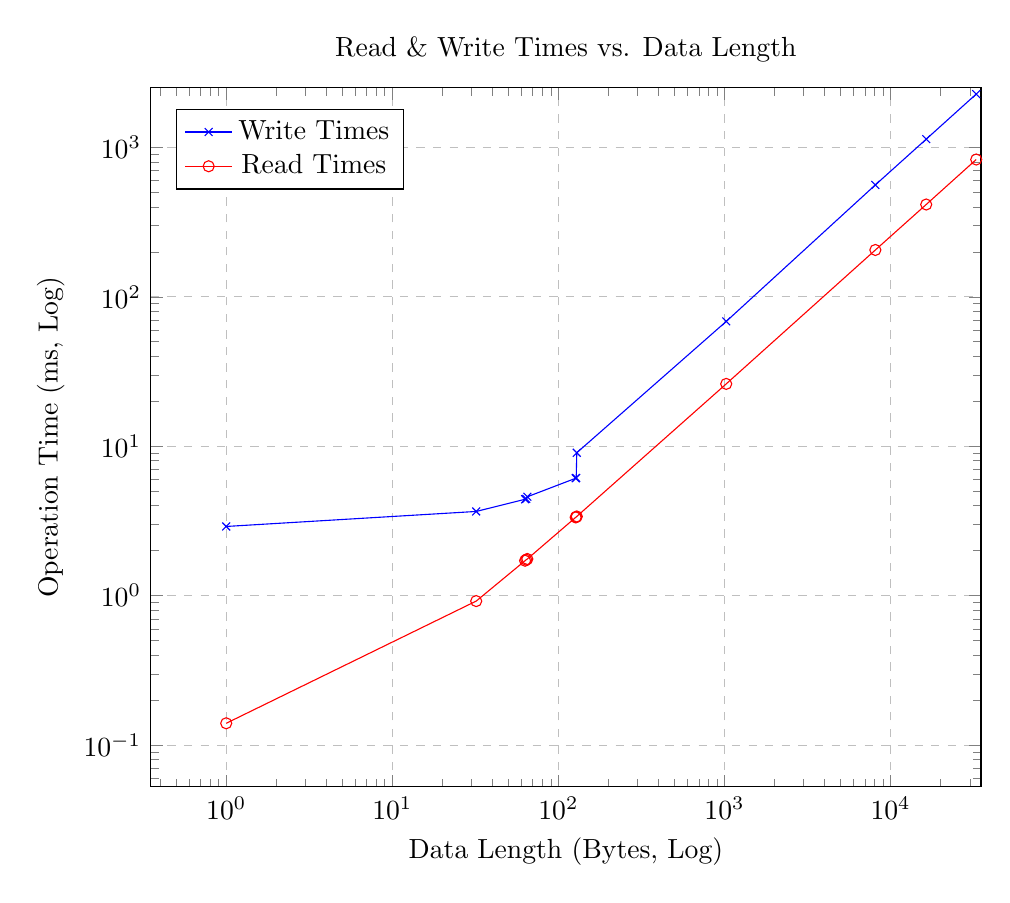
\begin{tikzpicture}
\begin{axis}[
    title={Read \& Write Times vs. Data Length},
    width=\textwidth,
    xmin=0, xmax=35000,
    xmode=log,
    xlabel={Data Length (Bytes, Log)},
    ymin=0, ymax=2500,
    ymode=log,
    ylabel={Operation Time (ms, Log)},
    ymajorgrids=true,
    xmajorgrids=true,
    legend pos=north west,
    grid style=dashed,
	]
	\addplot[
		color=blue,
		mark=x,
		]
		coordinates {
    			(1, 2.905)(32, 3.661)(63, 4.418)(64, 4.443)(65, 4.59)(127, 6.103)(128, 6.135)(129, 9.043)(1024, 68.409)(8096, 560.643)(16384, 1134)(32768, 2272)
		};
		\addlegendentry{Write Times}
	\addplot[
		color=red,
		mark=o,
		]
		coordinates {((1, 0.14)(32, 0.92)(63, 1.7133)(64, 1.74)(65, 1.76)(127, 3.34)(128, 3.36)(129, 3.39)(1024, 26.13)(8096, 205.68)(16384, 414.5)(32768, 829)
		};
		\addlegendentry{Read Times}
\end{axis}
\end{tikzpicture}

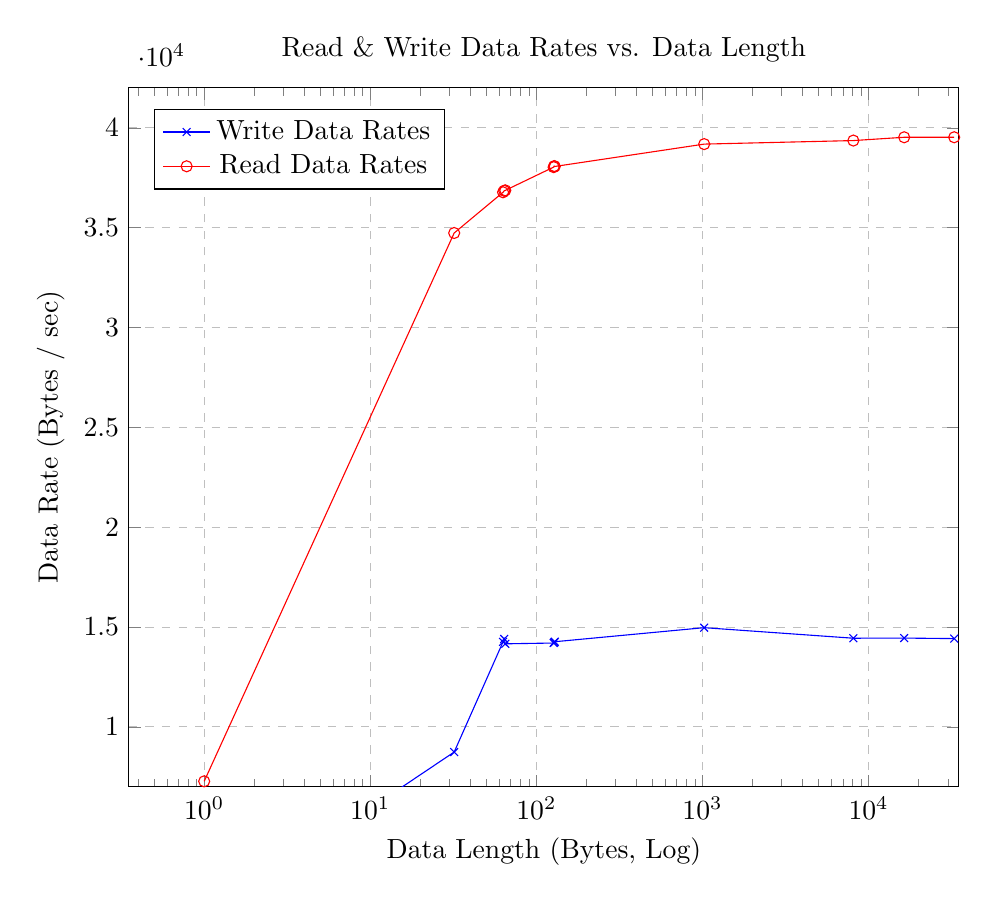
\begin{tikzpicture}
\begin{axis}[
    title={Read \& Write Data Rates vs. Data Length},
    width=\textwidth,
    xmin=0, xmax=35000,
    xmode=log,
    xlabel={Data Length (Bytes, Log)},
    ymin=7000, ymax=42000,
    ylabel={Data Rate (Bytes / sec)},
    ymajorgrids=true,
    xmajorgrids=true,
    legend pos=north west,
    grid style=dashed,
	]
	\addplot[
		color=blue,
		mark=x,
		]
		coordinates {
    			(1, 344)(32, 8741)(63, 14259)(64, 14404)(65, 14161)(127, 14200)(128, 14225)(129, 14265)(1024, 14969)(8096, 14441)(16384, 14448)(32768, 14422)
		};
		\addlegendentry{Write Data Rates}
	\addplot[
		color=red,
		mark=o,
		]
		coordinates {((1, 7275)(32, 34733)(63, 36771)(64, 36845)(65, 36868)(127, 38031)(128, 38083)(129, 38064)(1024, 39184)(8096, 39361)(16384, 39526)(32768, 39527)
		};
		\addlegendentry{Read Data Rates}
\end{axis}
\end{tikzpicture}
\end{center}

Using this collected data, the average data rate for writing to the EEPROM is about $12,740 \frac{Bytes}{sec}$. This is significantly lower than the data rate for \textit{reading} from the EEPROM, which is $35,356 \frac{Bytes}{sec}$; showing that reading is nearly three times faster than writing (on average).

Again, using this data, a generic expression can be generated to approximate the time required for writing and reading an arbitrary '$x$' amount of bytes. I began by deriving how long it takes \textit{per byte} of data, and I did this through solving the two simultaneous equations:

$$1\cdot b_w + 1\cdot p_w= 2.905\cdot 10^{-3}$$
$$32\cdot b_w + 1\cdot p_w = 3.661\cdot 10^{-3}$$

Using the data for my single and 32-byte write operations, and the fact that I know how many page transitions and bytes are written for each, these equations can be solved to find $b_w$ and $p_w$. $b_w$ and $p_w$ represent how long it takes to write one byte, and how long it takes to poll the EEPROM (respectively). I found the following:

$$b_w=0.02434\cdot 10^{-3}, p_w=2.8806\cdot 10^{-3}$$
$$b_r=0.024228\cdot 10^{-3}, p_r=0$$

Applying these to my formula results in a very accurate generic expression for both read and write times of $x$ number of arbitrary bytes:

$$T_{write}(x)\approx (x-64\cdot\floor*{\frac{x}{64}})*0.0243\cdot 10^{-3} + \floor*{\frac{x}{64}}*2.88\cdot 10^{-3}$$

$$T_{read}(x)\approx x * 0.024228\cdot 10^{-3}$$

For precision both of these formulas are accurate down to the millisecond, for both large and small numbers of bytes.
 
\section{Conclusion}
This was a wonderful lab to introduce $I^2C$. The EEPROM was intuitive, and although working around the page-latch limitation was somewhat challenging, it made having a complete understanding of the communication protocol a lot easier. Using the on-board peripheral for working with $I^2C$ made all of the communications very easy. I dont have a very clear understanding of the setup parameters available to me, but that's not an indictment on the lab. Other than that, the background information for this experiment was pretty straightforward.

Working with $I^2C$ has highlighted the problem of bidirectional buses. Even in this very simple program, the \textbf{SDA} line is used by both devices during a single operation. This is addressed by the $I^2C$ hardware implementation by having both lines be passively high, and only pulled low by the respective devices. This means that low lines are dominant, and any device who 'wants' the line to be high does nothing (as it's passively pulled high) and no short is generated on the device.

The consequences of solving bus contention this way is that the $I^2C$ protocol operates on slower transmission frequencies than similar protocols that use tri-stated drivers. This is because protocols like SPI, which use tri-state drivers, require more wires but can \textit{tell} devices to not drive the shared data line. This wouldn't work with $I^2C$ because the protocol allows for multi-master arbitration, and clock stretching (things not possible if an output was tri-stated).

\end{document}